\chapter{Внутреннее устройство и алгоритмы фаззинг-тестирования} \label{ch2}
	
% не рекомендуется использовать отдельную section <<введение>> после лета 2020 года
%\section{Введение} \label{ch2:intro}

%Глава посвящена более подробным примерам оформления текстово-графических объектов.
%
%В параграфе \ref{ch2:title-abbr} приведены примеры оформления многострочной формулы и одиночного рисунка. Параграф \ref{ch2:sec-abbr} раскрывает правила оформления перечислений и псевдокода. В параграфе \ref{ch2:sec-very-short-title} приведены примеры оформления сложносоставных рисунков, длинных таблиц, а также теоремоподобных окружений.
Глава посвящена подробному рассмотрению внутреннего устройства и алгоритмов, лежащих в основе фаззинг-тестирования. Особое внимание уделяется классификации методов фаззинга, которые различаются по уровню доступа к информации о тестируемой программе. Это разделение играет ключевую роль в выборе стратегии тестирования и определяет эффективность обнаружения уязвимостей. В главе также описываются различные методы fuzzing-тестирования, каждый из которых имеет свои особенности и предпочтительные области применения.


\section{Базовые этапы фаззинг-тестирования} \label{ch2:title-abbr} %название по-русски
\begin{enumerate}[label=\arabic*.]
	\item Определение целевой системы: Выбор программного обеспечения или системы, которая будет подвергнута тестированию.
	\item Определение входных данных: Анализ типов данных, обрабатываемых системой в нормальных условиях работы.
	\item Генерация fuzzing данных: Создание или модификация данных для генерации нестандартных входных значений, которые будут использоваться в тестах.
	\item Проведение теста с fuzzing данными: Подача сгенерированных данных в систему и наблюдение за её реакцией.
	\item Мониторинг поведения системы: Наблюдение за системой во время тестирования для выявления аномалий, сбоев и других нештатных ситуаций.
	\item Фиксация обнаруженных дефектов: Запись всех найденных проблем и уязвимостей в журнал дефектов для дальнейшего анализа.
	\item Анализ и устранение дефектов: Оценка выявленных уязвимостей и разработка решений для их исправления, направленных на повышение безопасности и надежности тестируемой системы [8].
\end{enumerate}

\newpage
На \firef{fig:fuzzer-works-ch2} приведён принцип работы фаззера.

\begin{figure}[ht] 
	\center
	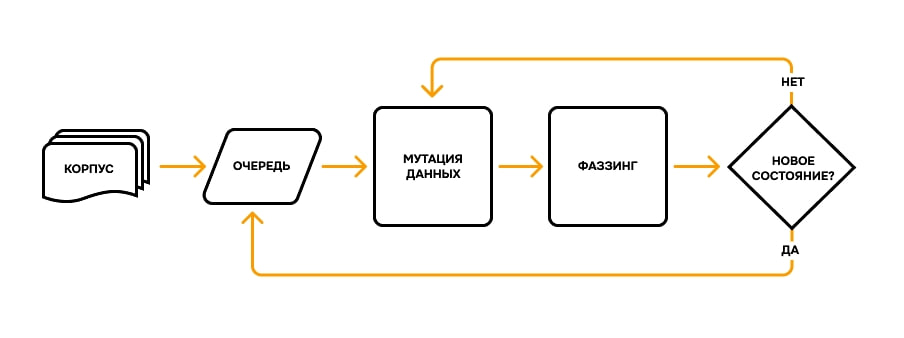
\includegraphics [scale=0.8] {my_folder/images/fuzzer_principe}
	\caption{Принцип работы фаззера} 
	\label{fig:fuzzer-works-ch2}  
\end{figure}

%%%%
%%		
%%  \input{...} commands are used only to sychronize some parts of the text with the author guide. Authors are free to type the text directly in .tex-files   
%%  \input{...} комманды используются только, чтобы синхронизировать части текта с рекомендациями авторам. Авторы  вольны вносить текст непосредственно в файл главы  
%%  
% \input{my_folder/tex/eq-Galois} % пример двух выравнивания двух формул в окружении align
%
%
%На \firef{fig:spbpu-new-bld-autumn-ch2} приведёна фотография Нового научно-исследовательского корпуса СПбПУ.
%
%	\begin{figure}[ht] 
%	\center
%	\includegraphics [scale=0.27] {my_folder/images/spbpu_new_bld_autumn}
%	\caption{Новый научно-исследовательский корпус СПбПУ \cite{spbpu-gallery}} 
%	\label{fig:spbpu-new-bld-autumn-ch2}  
%	\end{figure}
	


	
\section{Классификация методов фаззинга по уровню доступа к информации} \label{ch2:sec-abbr} %название по-русски
	Выделяют три вида фаззинга: \textit{фаззинг чёрного ящика, фаззинг серого ящика и фаззинг белого ящика}, в зависимости от того, сколько информации требуется фаззеру от тестируемой программы во время исполнения. Это разделение весьма условно, на практике, например, фаззеры белого ящика часто используют некоторые аппроксимации. Термин \textit{«черный ящик»}, обычно использующийся при тестировании программного обеспечения, в случае с фаззингом обозначает аналогичное: фаззер во время своей работы не получает никакой информации от тестируемой программы, он может взаимодействовать с программой только через ввод/вывод программы. Большинство традиционных фаззеров относят к этой категории. 
	\par
	\textit{Фаззинг белого ящика} — противоположность чёрного. Здесь программа анализирует внутреннее устройство тестируемой программы.
	Такой фаззер использует метод, который теоретически может исследовать все пути выполнения в тестируемой программе. В отличие от фаззинга черного ящика, фаззингу белого ящика требуется информация от тестируемой программы и она используется для руководства генерацией тестов. В частности, начиная исполнение с заданным конкретным входом, фаззер белого ящика сначала собирает символьные ограничения для всех условных операторов на пути исполнения. Следовательно, после одного исполнения такой фаззер объединяет все символьные ограничения с помощью конъюнкции для формирования ограничения пути. Затем фаззер белого ящика последовательно отрицает одно из ограничений и решает новое ограничение пути. Накладные расходы на фаззинг белого ящика обычно значительно превосходят расходы на фаззинг черного ящика. Это связано с тем, что реализации динамического символьного исполнения часто используют динамические инструменты и SMT-решатели, что весьма трудоёмко. Фаззинг серого ящика — что-то среднее между первыми двумя видами. 
	\par
	\textit{Фаззер серого ящика} может получать некоторую информацию о внутренней структуре тестируемой программы и/или её исполнении. Фаззеры серого ящика полагаются на приблизительную информацию, чтобы увеличить скорость и иметь возможность тестировать программу на большем количестве входных данных [3].
	
	На \firef{fig:white-gray-black-box-ch2} представлено сравнение подходов к тестированию ПО.
	
	\begin{figure}[ht] 
		\center
		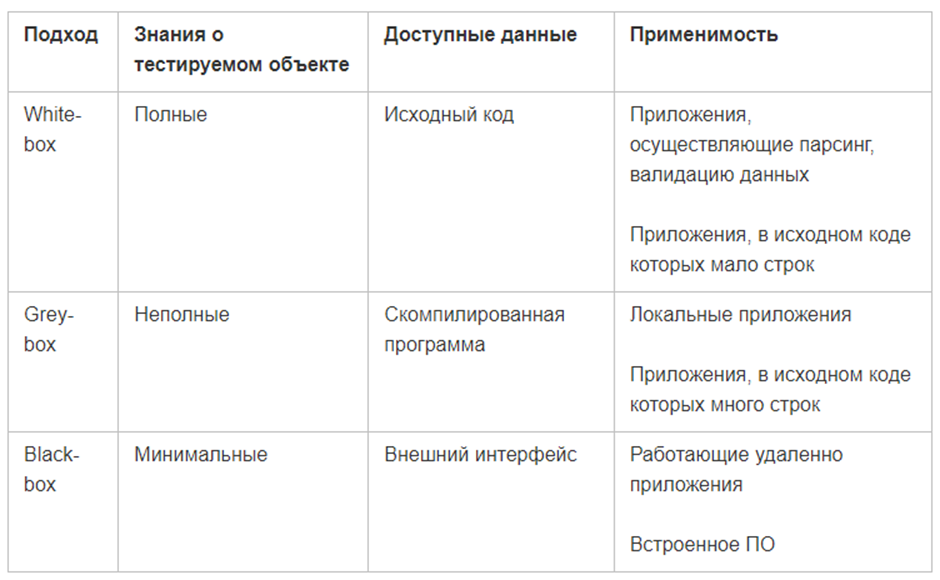
\includegraphics [scale=1] {my_folder/images/white-gray-black-box}
		\caption{Подходы к тестированию ПО [9]} 
		\label{fig:white-gray-black-box-ch2}  
	\end{figure}
	
%Название параграфа оформляется с помощью команды \verb|\section{...}|, название главы --- \verb|\chapter{...}|. 
%	
%
%\subsection{Название подпараграфа} \label{ch2:subsec-title-abbr} %название по-русски
%
%
%Название подпараграфа оформляется с помощью команды  \texttt{\textbackslash{}subsection\{...\}}.
%
%
%%\subsubsection{Название подподпараграфа} \label{ch2:subsubsec-title-abbr} %название по-русски
%	
%Использование подподпараграфов в основной части крайне не рекомендуется. В случае использования, необходимо вынести данный номер в содержание.	
%Название подпараграфа оформляется с помощью команды  \texttt{\textbackslash{}subsubsecti\-on\{...\}}.
%
%
%
%\input{my_folder/tex/enumeration} % правила использования перечислений	

	
%Оформление псевдокода необходимо осуществлять с помощью пакета \verb|algorithm2e| в окружении \verb|algorithm|. Данное окружение интерпретируется в шаблоне как рисунок. Пример оформления псевдокода алгоритма приведён на \firef{alg:AlgoFDSCALING}. 
%	
%	
%\input{my_folder/tex/pseudocode-agl-DTestsFDScaling} % пример оформления псевдокода алгоритма 	
%
%	
\section{Методы генерации данных fuzzing-тестирования} \label{ch2:sec-very-short-title} %название по-русски
\subsection{Случайное тестирование}\label{ch2:random-test}
Генерация начинается со случайных входных
данных в качестве аргументов, а затем используются некоторые дополнительные знания для получения новых входных данных. Одним
из основных представителей этой категории методов является случайное тестирование с обратной связью, которое улучшает генерацию
тестов за счёт полученной с предыдущих итераций обратной связи, которая направляет процесс создания входных данных на последующих
итерациях. Это позволяет снизить количество повторяющихся и/или
недопустимых входных данных, используемых для тестирования.
Инструменты для генерации тестов, использующие методы случайного тестирования, обладают преимуществами масштабируемости и простоты реализации, но используют много ресурсов на генерацию недопустимых, бесполезных (не улучшающих покрытие) входных данных ввиду случайной природы методов. Добавление обратной
связи позволяет нивелировать данный недостаток [3].

\subsection{Тестирование на основе поиска}\label{ch2:search-test}
При тестировании на основе поиска задача генерации тестов решается с
помощью алгоритмов поиска, например, генетических алгоритмов. В таком случае генерация входных данных формулируется как проблема поиска, множество возможных входных значений формирует пространство решений,
а метрика, которую хочется максимизировать, например, покрытие кода, кодируется как функция приспособленности. Таким образом, поиск
будет осуществляться с помощью выбранной функции приспособленности, которая представляет из себя эвристику, оценивающую, насколько
близко текущее решение к оптимальному. Руководствуясь функцией
приспособленности, алгоритм поиска итеративно выдаёт лучшие решение до тех пор, пока либо не будет найдено оптимальное решение, либо
не будет выполнено условие остановки (например, истечение выделенного на генерацию времени) [3].

\subsection{Символьное тестирование}\label{ch2:symbol-test}
Тестирование с помощью символьного исполнения — это аналитический подход, основанный на
правилах вывода. Он использует символьные переменные как входные
данные программы и представляет значения программных переменных
как символьные выражения, а путь исполнения — выражением над символьными переменными (ограничением пути). Символьное исполнение применяется для поиска всех возможных путей исполнения программы. Данный подход способен находить пути исполнения программы, которые вызывают ошибки, даже без компиляции. Для решения
ограничений пути, как правило, применяется SMT-решатель, который
вычисляет уже конкретные значения переменных, необходимых для того, чтобы поток исполнения пошёл по данному пути. Несмотря на очевидные преимущества и силу, этот подход обычно реализуется в мелком масштабе, так как в крупных проектах наблюдается значительный рост всех возможных путей исполнения, что требует серьёзных вычислительных ресурсов. Именно по этой причине этот подход только
недавно стал применяться для генерации тестов, хотя идея символьного
исполнения появилась в 70-х годах [3].
	
%\input{my_folder/tex/eq-equation-multilined} % пример оформления одиночной формулы в несколько строк
%
%\input{my_folder/tex/fig-spbpu-sc-four-in-one} % пример подключения 4х иллюстраций в одном рисунке
%
%%\input{my_folder/tex/fig-spbpu-whitehall-three-in-one} % пример подключения 3х иллюстрации в одном рисунке
%%
%%\input{my_folder/tex/fig-spbpu-main-bld-two-in-one} % пример подключения 2х иллюстраций в одном рисунке
%
%\input{my_folder/tex/tab-more-than-one-page} % пример подключения таблицы на несколько страциц
%
%
%\begin{table} [htbp]% Пример оформления таблицы
%	\centering\small
%	\caption{Пример представления данных для сквозного примера по ВКР \cite{Peskov2004}}%
%	\label{tab:ToyCompare}		
%		\begin{tabular}{|l|l|l|l|l|l|}
%			\hline
%			$G$&$m_1$&$m_2$&$m_3$&$m_4$&$K$\\
%			\hline
%			$g_1$&0&1&1&0&1\\ \hline
%			$g_2$&1&2&0&1&1\\ \hline
%			$g_3$&0&1&0&1&1\\ \hline
%			$g_4$&1&2&1&0&2\\ \hline
%			$g_5$&1&1&0&1&2\\ \hline
%			$g_6$&1&1&1&2&2\\ \hline		
%		\end{tabular}
%%	\caption*{\raggedright\hspace*{2.5em} Составлено (или/и рассчитано) по \cite{Peskov2004}} %Если проведена авторская обработка или расчеты по какому-либо источнику	
%	\normalsize% возвращаем шрифт к нормальному
%\end{table}
%
%
%
%%% please, before using, read the author guide carefully
%
%\input{my_folder/tex/tab-toy-context-minipage} % пример подключения minipage
%
%\input{my_folder/tex/fig-spbpu-new-bld-autumn-minipage} % пример подключения minipage
%
%
%
%
%\input{my_folder/tex/rules-theorem-like-expressions} 
%
%По аналогии с нумерацией формул, рисунков и таблиц нумеруются и иные текстово-графические объекты, то есть включаем в нумерацию номер главы, например: теорема 3.1. для первой теоремы третьей главы монографии. Команды \LaTeX{} выставляют нумерацию и форматирование автоматически. Полный перечень команд для подготовки текстово-графических и иных объектов находится в подробных методических рекомендациях \cite{spbpu-bci-template-author-guide}. 
%
%
%\input{my_folder/tex/rules-list-of-environments} % список некоторых окружений
%
%
%\input{my_folder/tex/theorem-example} %пример оформления теоремы
%
%
%\input{my_folder/tex/definition-example} %пример оформления определения
%
%
%Вместо теоремо-подобных окружений для вставки небольших текстово-графических объектов иногда используются команды. Типичным примером такого подхода является команда \verb|\footnote{text}|\footnote{Внимание! Команда вставляется непосредственно после слова, куда вставляется сноска (без пробела). Лишние пробелы также не указываются внутри команды перед и после фигурных скобок.}, где в аргументе \verb|text| указывают текст \textit{подстрочной ссылки (сноски)}.В них \textit{нельзя добавлять веб-ссылки или цитировать литературу}. Для этих целей используется список литературы. Нумерация сносок сквозная по ВКР без точки на конце выставляется в шаблоне автоматически, однако в каждом приложении к ВКР нумерация, зависящая от номера приложения, выставляется префикс <<П>>, например <<П1.1>> --- первая сноска первого приложения. 
%
%
%
%
%%\FloatBarrier % заставить рисунки и другие подвижные (float) элементы остановиться
%
%
%\section{Выводы} \label{ch2:conclusion}
%
%Текст заключения ко второй главе. Пример ссылок \cite{Article,Book,Booklet,Conference,Inbook,Incollection,Manual,Mastersthesis,Misc,Phdthesis,Proceedings,Techreport,Unpublished,badiou:briefings}, а также ссылок с указанием страниц, на котором отображены те или иные текстово-графические объекты  \cite[с.~96]{Naidenova2017} или в виде мультицитаты на несколько источников \cites[с.~96]{Naidenova2017}[с.~46]{Ganter1999}. Часть библиографических записей носит иллюстративный характер и не имеет отношения к реальной литературе. 
%
%Короткое имя каждого библиографического источника содержится в специальном файле \verb|my_biblio.bib|, расположенном в папке \verb|my_folder|. Там же находятся исходные данные, которые с помощью программы \texttt{Biber} и стилевого файла \texttt{Biblatex-GOST} \cite{ctan-biblatex-gost} приведены в списке использованных источников согласно ГОСТ 7.0.5-2008.
%Многообразные реальные примеры исходных библиографических данных можно посмотреть по ссылке \cite{ctan-biblatex-gost-examples}.
%
%Как правило, ВКР должна состоять из четырех глав. Оставшиеся главы можно создать по образцу первых двух и подключить с помощью команды \verb|\input| к исходному коду ВКР. Далее в приложении \ref{appendix-MikTeX-TexStudio} приведены краткие инструкции запуска исходного кода ВКР \cite{latex-miktex,latex-texstudio}.
%
%В приложении \ref{appendix-extra-examples} приведено подключение некоторых текстово-графических объектов. Они оформляются по приведенным ранее правилам. В качестве номера структурного элемента вместо номера главы используется <<П>> с номером главы. Текстово-графические объекты из приложений не учитываются в реферате.
%
%
%
%%% Вспомогательные команды - Additional commands
%%
%%\newpage % принудительное начало с новой страницы, использовать только в конце раздела
%%\clearpage % осуществляется пакетом <<placeins>> в пределах секций
%\newpage\leavevmode\thispagestyle{empty}\newpage % 100 % начало новой страницы